\chapter{Redes Neuronales y Modelos Generativos}\label{chap:redes-neuronales-y-modelos-generativos}
{
Este capítulo introducirá los conceptos esenciales acerca de los modelos generativos. Para ello, se empezará por definir lo qué es una red neuronal.
\section{Redes Neuronales}\label{sec:redes-Neuronales}
{
En el último tiempo se ha visto un auge en el uso de las redes neuronales en diversas áreas de la ciencia y la tecnología. Esto se debe a que las redes neuronales han demostrado ser muy efectivas en la resolución de problemas complejos, como la clasificación de imágenes, el procesamiento de lenguaje natural, y la generación de texto e imágenes, entre otros.

En este capítulo, se introducirán los conceptos básicos de las redes neuronales, aunque no se profundizará en los detalles de su funcionamiento. Para ello, se recomienda al lector revisar la literatura especializada en el tema.

Una red neuronal (feedforward) es simplemente una composición de funciones lineales y no lineales. Más precisamente, dado un número natural $L$, el cuál denominaremos como la \emph{profundidad} de la red neuronal, se definen las funciones lineales $g^{(\ell)}_{\vth_\ell}$, con $\ell \in \left\{ 1, \ldots, L \right\}$. Cada una de estas funciones se encuentran parametrizadas por $\vth_\ell = (\vW_\ell, b_\ell)$, donde $\vW_\ell \in \R^{d_{\ell} \times d_{\ell-1}}$ corresponden a los \emph{pesos} y $b_\ell \in \R^{d_\ell}$ corresponde al \emph{bias}. Estas funciones se definen de la siguiente manera:
\begin{align*}
    g^{(\ell)}_{\vth_\ell} \colon \R^{d_{\ell-1}} & \to \R^{d_\ell}                                                        \\
    \vx_\ell                                      & \mapsto g^{(\ell)}_{\vth_\ell}(\vx_\ell) = \vW_\ell \vx_\ell + b_\ell,
\end{align*}
que, junto con una familia de funciones no-lineales $\sigma^{(\ell)},\ \ell \in \left\{ 1, \ldots, L \right\}$, a las cuales llamaremos por \emph{funciones de activación}, se pueden componer para formar una red neuronal:
% , se pueden componer para formar una red neuronal:
\begin{equation}
    f_{\vth}(\vx) = \sigma^{(L)} \circ g^{(L)}_{\vth_L} \circ \sigma^{(L-1)} \circ g^{(L-1)}_{\vth_{L-1}} \circ \cdots \circ \sigma^{(1)} \circ g^{(1)}_{\vth_{1}}(\vx).
\end{equation}

A este tipo de modelos se les suele representar como grafos dirigidos acíclicos, describiendo cómo las funciones se encuentran compuestas entre sí. En la Figura~\ref{fig:ejemplo-red-neuronal} se muestra un ejemplo de una red neuronal con dos capas ocultas.

\begin{figure}[htbp]
    \centering
    % \missingfigure{Ejemplo de una red neuronal}
    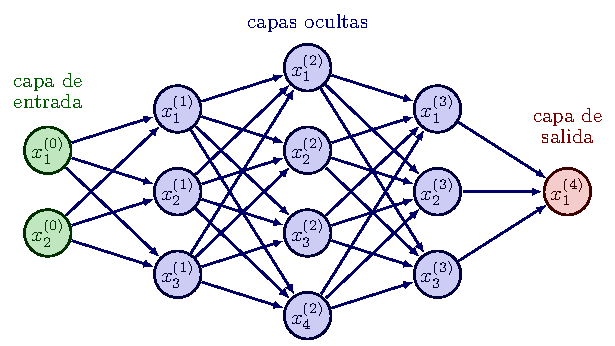
\includegraphics[width=0.5\textwidth]{img/neural_network/neural_network_feed_forward.pdf}
    \caption{caption}
    \label{fig:ejemplo-red-neuronal}
\end{figure}


donde $\sigma^{(\ell)}$ corresponde a la función de activación de la capa $\ell$, la cuál generalmente es una función no-lineal.

\section{Redes Neuronales Feedforward}\label{sec:redes-neuronales-feedforward}
{
    A pesar del éxito que han tenido las redes neuronales, y que se puede pensar que son modelos muy complejos, en realidad, las redes neuronales son modelos muy simples. La idea detrás de las redes neuronales es la de aproximar alguna función objetivo $f^\ast$, con la intención de realizar alguna clasificación o regresión. Sin embargo, la tarea puede ser más amplia, como el objetivo de esta sección: que la red aprenda a generar muestras realistas de algún conjunto de datos.


}



Las redes neuronales feedforward, también llamadas perceptrones multicapa, son los modelos de \textit{deep learning} por excelencia. La tarea de estas redes es la de aproximar alguna función objetivo $f^\ast$, con la intención de realizar alguna clasificación o regresión, aunque la tarea puede ser más amplia, como el objetivo de esta sección: que la red aprenda a generar muestras realistas de algún conjunto de datos.

A estos modelos se les llama redes neuronales porque están inspiradas en la forma en que las neuronas del cerebro se comunican entre sí: en como una neurona recibe una señal, la procesa, y luego envía esta señal a otras neuronas para procesar información aún más compleja. Esta analogía se puede ver en la Figura~\ref{fig:ejemplo-red-neuronal}.

% \begin{figure}[htbp]
%     \centering
%     \missingfigure{Ejemplo de una red neuronal}
%     % \includegraphics[width=0.5\textwidth]{}
%     \caption{caption}
%     \label{fig:ejemplo-red-neuronal}
% \end{figure}


% Estos modelos se llaman feedforward porque la información $\vx$ fluye a través de la red. Mientras que se les denomina redes porque suelen estar representadas por la combinación de varias funciones distintas. Usualmente se les ilustra como grafos dirigidos acíclicos, describiendo cómo las funciones se encuentran compuestas entre sí.

Formalmente, las redes neuronales se definen como una composición de funciones no-lineales $f^{(\ell)}_{\vth_\ell}$. Cada función $f^{(\ell)}_{\vth_\ell}$ se encuentra parametrizada por $\vth_\ell = (\vW_\ell, b_\ell)$, donde $\vW_\ell \in \R^{d_{\ell} \times d_{\ell-1}}$ corresponden a los pesos y $b_\ell \in \R^{d_\ell}$ corresponde al bias. Estas redes se encuentran definidas de la siguiente manera:
\begin{align*}
    f^{(\ell)}_{\vth_\ell} \colon \R^{d_{\ell-1}} & \to \R^{d_\ell}                                                                         \\
    \vx_\ell                                      & \mapsto f^{(\ell)}_{\vth_\ell}(\vx_\ell) = \sigma^{(\ell)}(\vW_\ell \vx_\ell + b_\ell),
\end{align*}
donde $\sigma^{(\ell)}$ corresponde a la función de activación de la capa $\ell$, la cuál generalmente es una función no-lineal.

Una \emph{red neuronal} $f_{\vth}$ se define como la composición de funciones no-lineales $f^{(\ell)}_{\vth_{\ell}}$,
es decir,
\begin{equation}
    f_{\vth}(\vx) = f^{(L)}_{\vth_{L}} \circ f^{(L-1)}_{\vth_{L-1}} \circ \cdots \circ f^{(1)}_{\vth_{1}}(\vx),
\end{equation}
donde los parámetros de la red $f_{\vth}$ son $\vth = (\vW_1, b_1, \vW_2, b_2, \ldots, \vW_L, b_L)$. Cada una de las funciones no-lineales $f^{(\ell)}_{\vth_{\ell}}$ se les llama la capa $\ell$-ésima de la red, siendo el número de capas $L$ la profundidad de la red.

A partir de la ecuación anterior, se puede ver que las funciones de activación $\sigma^{(\ell)}$ deben de ser funciones no-lineales. Pues si no lo fueran, entonces la red sería una composición de funciones lineales, lo que resulta en una única función lineal. El problema que tendría con esto es que no habría ninguna ganancia con hacer la red más profunda, pues todo colapsaría a una única capa.\FM{Este parrafo se pude quitar, no es tan importante}

Para cumplir con el objetivo de \emph{aprender}, la red neuronal debe de minimizar una función de pérdida $\cL(\vth; \vx, \vy)$, que mide el error que ha cometido la red neuronal al predecir una salida $\vy$ a partir de una entrada $\vx$ utilizando el parámetro $\vth$. Un ejemplo de función de pérdida puede ser el error cuadrático medio:
\begin{equation}
    \cL(\vth; \vx, \vy)
    = \frac{1}{N}
    \sum_{i=1}^{N}
    \|\vy_i - f_{\vth}(\vx_i)\|^2.
\end{equation}
Por tanto, para que la red neuronal aprenda, se debe de resolver el siguiente problema de optimización:
% de forma que la red \emph{aprenda} se reduce en intentar resolver el siguiente problema de optimización:
\begin{align*}
    \min_{\vth} \mathcal{L}(\vth; \vx, \vy)
    %  & = \min_{\vth} \mathcal{L}(\vth; \vx, \vy)            \\
    %   & = \min_{\vth} \mathcal{L}(\vth; \vx, f_{\vth}(\vx)).
\end{align*}


% . Cada función $f^{(\ell)}_{\vth_\ell}$ se encuentra parametrizada por $\vth_\ell = (\vW_\ell, b_\ell)$, y la red neuronal $f_\vth$ se encuentra parametrizada por $\vth = (\vW_{1}, b_1, \ldots, \vW_L, b_L)$. Escrito en términos matemáticos:

% La red neuronal $f_\vth$ correspondería entonces a una composición de funciones no-lineales $f^{(\ell)}_{\vth_\ell}$, donde cada función $f^{(\ell)}_{\vth_\ell}$ se encuentra parametrizada por $\vth_\ell = (\vW_\ell, b_\ell)$, y la red neuronal $f_\vth$ se encuentra parametrizada por $\vth = (\vW_{1}, b_1, \ldots, \vW_L, b_L)$. Escrito en términos matemáticos:




% La red neuronal $f_\theta$ se encuentra parametrizada por $\theta = (W_{1}, b_1, \ldots, W_L, b_L)$. Escrito en términos matemáticos:
% y la red neuronal $f_\theta$ se encuentra parametrizada por $\theta = (W_{1}, b_1, \ldots, W_L, b_L)$. Escrito en términos matemáticos:

% Los perceptrones multicapa (MLP) corresponden a una parte fundamental al área del Deep Learning. El objetivo de un MLP es el de aproximarse a alguna función $f^\ast$. Por ejemplo, para un clasificador, $y = f^\ast(\vx)$ mapea una entrada $\vx$ a una categoría $y$. Una MLP define
%  Un MLP define una familia de funciones parametrizadas por $\theta$ que denotaremos como $f_\theta$. Por ejemplo, un MLP con una sola capa oculta y una función de activación $\sigma$ es definido como:
% Una red neuronal puede ser entendida como una función $f_\theta$, que es definida por medio de composición de funciones no-lineales $f^{(\ell)}_{\theta_\ell}$. Cada función $f^{(\ell)}_{\theta_\ell}$ se encuentra parametrizada por $\theta_\ell = (W_\ell, b_\ell)$, y la red neuronal $f_\theta$ se encuentra parametrizada por $\theta = (W_{1}, b_1, \ldots, W_L, b_L)$. Escrito en términos matemáticos:
% \begin{equation}
%     f_\theta(x) = f^{(L)}_{\theta_{L}} \circ f^{(L-1)}_{\theta_{L-1}} \circ \cdots \circ f^{(1)}_{\theta_{1}} (x).
% \end{equation}

% Cada función $f^{(\ell)}_{\theta_{\ell}}$ está definida desde un espacio de partida $\R^{d_{\ell-1}}$ a un espacio de llegada $\R^{d_\ell}$. Estas funciones se encuentran definidas por medio de:
% \begin{equation}
%     f^{(\ell)}_{\theta_{\ell}} (x_\ell) = \sigma^{(\ell)} (W_\ell \cdot x_\ell + b_\ell),
% \end{equation}
% donde $x_\ell \in \R^{d_{\ell-1}}$ es la entrada de la función, $\sigma^{(\ell)}$ es una función no-lineal, también llamada \emph{función de activación}, $\theta_\ell = (W_\ell, b_\ell)$ son los parámetros de la función, con $W_\ell \in \R^{d_{\ell} \times d_{\ell-1}}$ los \emph{pesos} y $b_\ell \in \R^{d_\ell}$ el \emph{bias}.

\section{Redes Neuronales Convolucionales}\label{sec:redes-neuronales-convolucionales}
{
    \FM[inline]{Escribir! (será necesario?)}
}  % end of sec. Redes Neuronales Convolucionales

\section{Redes Generativas Adversarias}\label{sec:redes-generativas-adversarias-GAN}
{
% Analogía ladron-policía
Comencemos imaginando la siguiente situación\footnote{Este ejemplo es una adaptación y fue inspirado de \cite[min. 4:32]{santana2017creando}}:
% Supongamos que hay un ladrón que desea engañar a un policía entregándole un billete falso. El ladrón, que es un inexperto, le entrega una servilleta, con una cara dibujada en ella, y que en el otro lado de la servilleta tiene escrito: ``\emph{esto vale un millón de dólares}''. El policía, que ha sido entrenado en la detección de billetes falsos, revisa el billete para comprobar que, efectivamente, es un billete falso. Sin embargo, en vez de enviar a la cárcel al ladrón, lo que hace es decirle al ladrón cuales fueron sus fallos, y de qué manera puede este mejorar en sus falsificaciones. Por su parte, el policía también se entrena más y más en la detección de billetes falsos, pues puede que en algún momento, el ladrón se vuelva tan bueno en la elaboración de billetes falsos, que llegue a engañar al policía con uno de sus billetes.

% Definición de las GANs, como un problema de clasificación reales-falsas
% Las redes generativas adversarias (GANs) son un tipo de arquitectura de redes neuronales que se basan en la analogía del ladrón y el policía. En este caso, el ladrón es una red neuronal generativa $G$, que se encarga de generar muestras que parezcan reales, y el policía es una red neuronal discriminativa $D$, que se encarga de clasificar las muestras como reales o falsas. En este caso, la red generativa $G$ se entrena para engañar a la red discriminativa $D$, y la red discriminativa $D$ se entrena para detectar las muestras generadas por la red generativa $G$.
\begin{quotation}
    \textit{Supongamos que hay un ladrón que desea engañar a un policía entregándole un billete falso. El ladrón, que es un inexperto, le entrega una servilleta, con una cara dibujada en ella, y que en el otro lado de la servilleta tiene escrito: ``\emph{esto vale un millón de dólares}''. El policía, que ha sido entrenado en la detección de billetes falsos, revisa el billete para comprobar que, efectivamente, es un billete falso.}

    \textit{Sin embargo, en vez de enviar a la cárcel al ladrón, lo que hace es decirle al ladrón cuales fueron sus fallos, y de qué manera puede este mejorar en sus falsificaciones. Por su parte, el policía también se entrena más y más en la detección de billetes falsos, pues puede que en algún momento, el ladrón se vuelva tan bueno en la elaboración de billetes falsos, que llegue a engañar al policía con uno de sus billetes.}
\end{quotation}

El marco de las Redes Generativas Adversarias (GAN), introducidos por \cite{goodfellow2014generative}, es en esencia, la analogía del ladrón y el policía.
La GAN define un juego donde el objetivo de la \emph{generadora} (el ladrón) es la de generar muestras que parezcan reales, mientras que el objetivo de la \emph{discriminadora} (el policía) es el de clasificar las muestras como verdaderas o falsas.
En este caso, la generadora se entrena para engañar a la discriminadora, y la discriminadora se entrena para detectar la falsedad de las muestras generadas.

Más formalmente, desde el punto de vista de la teoría de juegos, la GAN se define como un juego de dos jugadores: una generadora $\Prob_G$, donde su conjunto de estrategias es $\ProbSpace[\cX]$ (donde $\cX$ es el conjunto de referencia, e.g. $\cX=[0, 1]^{n_1\times n_2}$ para un conjunto de imágenes), y una discriminadora $\Prob_D(\dd y \mid x)$, donde su conjunto de estrategias es el conjunto de kernels Markovianos.\FM{Creo que aquí podría haber un punto aparte en vez de un punto seguido.} Con esto, la GAN es un juego de suma cero con la siguiente función valor objetivo:
\begin{equation}
    \label{eq:gan-objective}
    V(\Prob_G, \Prob_D)
    = \Exp_{X\sim\Prob_G}{\Exp_{Y \sim \Prob_D(\dd y \mid X)} \left[ \ln Y \right]}
    + \Exp_{\tilde X\sim\Prob_G}{\Exp_{Y \sim \Prob_D(\dd y \mid \tilde X)} \left[ \ln (1 - Y) \right]},
\end{equation}
donde la generadora busca minimizar la función valor, mientras que la discriminadora busca maximizar esta cantidad. El objetivo final de la generadora es el de encontrar una distribución $\Prob_G$ tal que se aproxime a una distribución de referencia $\Prob_X \in \ProbSpace[\cX] $. Por el otro lado, el objetivo de la discriminadora es el de clasificar las muestras verdaderas y falsas, asignándole valores cercano a 1 y 0 respectivamente.

% En la práctica, la forma de implementar la generadora es a través de un \emph{modelo generativo de espacio latente}. Esto es,
% \begin{equation}
%     \Prob_G (\dd x) \eqdef \int_\cZ \Prob_G(\dd x \mid z) \; \Prob_Z \left( \dd z\right),
% \end{equation}
% donde $\cZ$ es el espacio de las variables latentes, y $\Prob_Z \in \ProbSpace[\cZ] $ es la distribución del espacio latente (típicamente se utiliza distribución Gaussiana o Uniforme). Por simplicidad, el modelo generativo $\Prob_G (\dd x \mid z)$ se mapea de forma determinista a través de $\Prob_G (\dd x \mid z) = \delta_{G(z)}(\dd x)$, a través de una función $G\colon \cZ \to \cX$.

El siguiente teorema nos habla acerca de la naturaleza del discriminador óptimo:

\begin{theorem}[El discriminador óptimo calcula la divergencia de JS]
    \label{thm:gan-optimal-discriminator}
    Para cualquier estrategia de generador $\Prob_G$ fijo, existe un único discriminador óptimo $\Prob_D^\ast$ que maximiza la función objetivo \eqref{eq:gan-objective}, el cuál toma una forma determinista por medio de $\Prob_D^\ast(\dd y \mid x) = \delta_{D^\ast(x)}(\dd y)$, donde $D^\ast(x) = \dv{\Prob_X}{(\Prob_G+\Prob_X)}$. En tal caso, la función valor toma la siguiente forma:
    \begin{equation}
        V(\Prob_G, \Prob_D^\ast) = \JS{\Prob_X}{\Prob_G} - 2 \ln 2.
    \end{equation}
\end{theorem}

Este teorema nos dice que el discriminador óptimo es aquel que calcula la divergencia de Jensen-Shannon entre la distribución de referencia $\Prob_X$ y la distribución generada $\Prob_G$, salvo una constante. Además, nos dice que el discriminador toma una forma determinista, de forma que bastaría con buscar una función (como por ejemplo, una red neuronal) $D\colon\cX\to [0, 1]$ tal que la aproxime.

\begin{proof}
    Dado $X \sim \Prob_X$, por la desigualdad de Jensen se tiene que:
    \begin{equation}
        \Exp_{Y \sim \Prob_D \left( \dd y \mid X \right)} \left[ \ln Y \right]
        \leq \ln \left( \Exp_{Y \sim \Prob_D \left( \dd y \mid X \right)} \left[ Y \right] \right),
    \end{equation}
    el cuál es análogo para $\tilde X \sim \Prob_G$. Por el lema de Doob\FM{Agregar cita! Quizás se podría poner el del JSM o el lema directo}, se sabe que existe una función $D \colon \cX \to [0, 1]$ tal que $\Exp_{Y \sim \Prob_D \left( \dd y \mid X \right)} \left[ Y \right]
        = D(X)$,
    % \begin{equation}
    %     \Exp_{Y \sim \Prob_D \left( \dd y \mid X \right)} \left[ Y \right]
    %     = D(X),
    % \end{equation}
    es decir, que el discriminador toma una forma determinista $\Prob_D \left( \dd y \mid x \right) = \delta_{D(x)}(\dd y)$,
    % centrada en $D(X)$,
    y por tanto, se tiene que:
    \begin{equation}
        V(\Prob_G, \Prob_D) \leq \Exp_{X \sim \Prob_X} \Big[ \ln D(X) \Big] + \Exp_{\tilde X \sim \Prob_G} \Big[ \ln \qty\big(1 - D(\tilde X)) \Big],
    \end{equation}
    y dado que la parte derecha de la desigualdad es una cota superior de la función valor, s.p.g. se puede asumir que el discriminador toma una forma determinista en el óptimo. En tal caso, la función valor toma la forma del lado derecho de la desigualdad anterior.
    % \begin{equation}
    %     V(\Prob_G, \Prob_D) = \Exp_{X \sim \Prob_X} \Big[ \ln D(X) \Big] + \Exp_{\tilde X \sim \Prob_G} \Big[ \ln \qty\big(1 - D(\tilde X)) \Big].
    % \end{equation}

    Tomando $\Prob = \Prob_X + \Prob_G$, es claro que $\Prob_X \ll \Prob$ y $\Prob_G \ll \Prob$, y por tanto, existen las derivadas de Radon-Nikodym:
    \begin{align*}
        \rho_X & = \dv{\Prob_X}{\Prob}, & \rho_G & = \dv{\Prob_G}{\Prob},
    \end{align*}
    donde claramente $\rho_X + \rho_G = 1$. En tal caso, la función valor toma la siguiente forma:
    \begin{equation}
        \label{eq:gan-objective-2}
        V(\Prob_G, \Prob_D) = \int_\cX \big[ \rho_X(x) \ln D(x) + \rho_G(x) \ln \qty(1 - D(x)) \big] \; \Prob(\dd x).
    \end{equation}
    Notemos que la función $y \mapsto a \ln y + b \ln(1-y)$ alcanza su máximo en $y^\ast = \frac{a}{a+b}$, y por tanto, la función $D^\ast$ que maximiza la función valor es:
    \begin{equation}
        D^\ast = \frac{\rho_X}{\rho_X + \rho_G} = \dv{\Prob_X}{(\Prob_X + \Prob_G)} .
    \end{equation}
    Por otro lado, si evaluamos $D^\ast$ en la función valor \eqref{eq:gan-objective-2}, se tiene que:
    \begin{align*}
        V(\Prob_G, \Prob_D^\ast)
         & = \Exp_{X \sim \Prob_X} \left[ \ln \dv{\Prob_X}{\Prob}(X) \right] + \Exp_{\tilde X \sim \Prob_G} \left[ \ln \dv{\Prob_G}{\Prob}(\tilde X) \right] \\
         & = \KL{\Prob_X}{\frac{\Prob_X + \Prob_G}{2}} - \ln 2 + \KL{\Prob_G}{\frac{\Prob_X + \Prob_G}{2}} - \ln 2                                           \\
         & = \JS{\Prob_X}{\Prob_G} - 2 \ln 2,
    \end{align*}
    lo que concluye la demostración.
\end{proof}

Dado que para cada generador $\Prob_G$ existe un único discriminador óptimo $\Prob_D^\ast$, entonces tiene sentido definir la siguiente función:
\begin{equation}
    C(\Prob_G) \eqdef V(\Prob_G, \Prob_D^\ast) = \JS{\Prob_X}{\Prob_G} - 2 \ln 2.
\end{equation}
El siguiente teorema nos dice que existe un único generador óptimo $\Prob_G^\ast$ que minimiza la función $C(\Prob_G)$, y que este corresponde a la distribución de referencia $\Prob_X$:

\begin{theorem}
    El mínimo global de la función $C(\Prob_G)$ se alcanza en $\Prob_G^\ast = \Prob_X$, y el valor mínimo es $C(\Prob_X) = - \ln 4$.
\end{theorem}

\begin{proof}
    Por el Teorema anterior, se tiene que:
    \begin{align*}
        \min_{\Prob_G} \max_{\Prob_D} V(\Prob_G, \Prob_D)
         & = \min_{\Prob_G} V(\Prob_G, \Prob_D^\ast)         \\
         & = \min_{\Prob_G} C(\Prob_G)                       \\
         & = \min_{\Prob_G} \JS{\Prob_X}{\Prob_G} - 2 \ln 2.
    \end{align*}
    Como la divergencia de Jensen-Shannon es estrictamente positiva si $\Prob_G \neq \Prob_X$, y nula si $\Prob_G = \Prob_X$, entonces se tiene que el mínimo global de la función $C(\Prob_G)$ se alcanza en $\Prob_G^\ast = \Prob_X$, y el valor mínimo es $C(\Prob_X) = - \ln 4$. Esto concluye la demostración.
\end{proof}

En la práctica, la forma de implementar la generadora es a través de un \emph{modelo generativo de espacio latente}. Esto es,
\begin{equation}
    \Prob_G (\dd x) \eqdef \int_\cZ \Prob_G(\dd x \mid z) \; \Prob_Z \left( \dd z\right),
\end{equation}
donde $\cZ$ es el espacio de las variables latentes, y $\Prob_Z \in \ProbSpace[\cZ] $ es la distribución del espacio latente (típicamente se utiliza la distribución Gaussiana o Uniforme).

Por simplicidad, el modelo generativo $\Prob_G (\dd x \mid z)$ se mapea de forma determinista a través de $\Prob_G (\dd x \mid z) = \delta_{G(z)}(\dd x)$, a través de una función $G\colon \cZ \to \cX$, la cuál la estimaremos a través de una red neuronal $G_\theta$. Por otro lado, el Teorema~\ref{thm:gan-optimal-discriminator} nos dice que, en el óptimo, el discriminador toma una forma determinista, de forma que bastaría con sólo buscar una función $D\colon\cX\to [0, 1]$, la cual la estimaremos a través de una red neuronal $D_\varphi$.
%  tal que la aproxime. Para ello, utilizaremos una red neuronal $D_\phi$.
% el discriminador óptimo toma una forma determinista, de forma que bastaría con sólo buscar una función $D\colon\cX\to [0, 1]$ tal que la aproxime. En la práctica, esta función $D$ se implementa a través de una red neuronal $D_\phi$.

\FM{Agregar una explicación de las funciones de pérdida para este caso, explicar qué cosas buscan minimizar/maximizar y describir el algoritmo de entrenamiento.}
De esta forma, el algoritmo para estimar los parámetros $\theta$ y $\varphi$ de la generadora y la discriminadora, respectivamente, es el siguiente:

\begin{algorithm}[tbhp]
    \caption{GAN}\label{alg:GAN}
    \begin{algorithmic}
        \Require Tamaño del batch $N$ y número de iteraciones para el discriminador $N_d$.
        % Penalization coefficients $\lambda_1, \lambda_2 > 0$, the number of critic iterations $n_{\text{critic}}$, the batch size $m$.
        \State Inicializar los parámetros de la generadora $G_\theta$ y la discriminadora $D_\varphi$.
        % Initialize the parameters of the encoder $Q_\phi$, \\generator/decoder $G_\theta$ and the critic function $f_\omega$.
        \While{$\theta$ no ha convergido}
        \For{$t=0,\ldots,N_d$}
        \State Muestrear $\{x_i\}_{i=1}^{N} \sim \Prob_X$ desde el conjunto de entrenamiento.
        \State Muestrear $\{z_i\}_{i=1}^{N} \sim \Prob_Z$ desde el espacio latente.
        \State $\cL_{\mathrm{disc}} \gets -\frac{1}{N}\sum_{i=1}^{N} \Big[ \ln D_\varphi(x_i) + \ln \qty\big(1 - D_\varphi(G_\theta(z_i))) \Big]$
        \State Actualizar $D_\varphi$ por medio de descenso de gradiente en $\pdv{\varphi} \cL_{\mathrm{disc}}$.
        % \State $\widehat W^{(1)}_{\omega}(\theta) \gets \frac{1}{m}\sum_{i=1}^{m} f_\omega(x_i) - \frac{1}{m}\sum_{i=1}^{m} f_\omega(G_\theta(z_i))$
        % \State $\cL_{\text{critic}} \gets -\widehat W^{(1)}_{\omega}(\theta) + \lambda_1 \cP(f_\omega)$
        % \State Update $f_\omega$ by descending $\pdv{\omega} \cL_{\text{critic}}$.
        \EndFor
        \State Muestrear $\{z_i\}_{i=1}^{N} \sim \Prob_Z$ desde el espacio latente.
        \State $\cL_{\mathrm{gen}} \gets \frac{1}{N}\sum_{i=1}^{N} \ln \qty\big(1 - D_\varphi(G_\theta(z_i)))$
        \State Actualizar $G_\theta$ por medio de descenso de gradiente en $\pdv{\theta} \cL_{\mathrm{gen}}$.
        % \State Update $G_\theta$ by descending $\pdv{\theta} \widehat W^{(1)}_{\omega}(\theta)$.
        % \State Sample $\tilde z_i \sim Q_\phi(dz | x_i)$ for $i=1,\ldots, m$.
        % \State $\widehat W^{(2)}_{\phi}(\theta) \gets \frac{1}{m}\sum_{i=1}^{m} |x_i - G_\theta(\tilde z_i)|$
        % \State $\cL_{\text{WAE}} \gets \widehat W^{(2)}_{\phi}(\theta) + \lambda_2 \cD(\{z_i\}_{i=1}^{m}, \{\tilde z_i\}_{i=1}^{m})$
        % \State Update $Q_\phi$ by descending $\pdv{\phi} \cL_{\text{WAE}}$.
        % \State Update $G_\theta$ by descending $\pdv{\theta} \widehat W^{(2)}_{\phi}(\theta)$.
        \EndWhile
    \end{algorithmic}
\end{algorithm}

\begin{remark}
    Notemos que este algoritmo lo primero que hace intentar encontrar el óptimo de $\max_D V(G, D)$, el cuál proporciona una aproximación para la divergencia de Jensen-Shannon entre $\Prob_X$ y $\Prob_G$. Luego, se actualiza la generadora $G$ para minimizar la divergencia de Jensen-Shannon entre $\Prob_X$ y $\Prob_G$. Con este procedimiento, la generadora $G$ se aproxima a la distribución de referencia $\Prob_X$ utilizando la divergencia de Jensen-Shannon.
\end{remark}






% El objetivo entonces de la generadora es el de maximizar la función objetivo, mientras que el objetivo de la discriminadora es el de minimizar la función objetivo. En otras palabras, la generadora se entrena para engañar a la discriminadora, y la discriminadora se entrena para clasificar la falsedad de las muestras generadas por la generadora.




% Las Redes Generativas Adversarias (GAN por sus siglas en inglés) son un tipo de arquitectura que se componen de dos partes: un generador $G$ y un discriminador $D$. El objetivo de la generadora $G$ es el de generar muestras que parezcan reales, mientras que el objetivo del discriminador $D$ es el de clasificar las muestras como reales o falsas. En este caso, la red generativa $G$ se entrena para engañar a la red discriminativa $D$, y la red discriminativa $D$ se entrena para detectar las muestras generadas por la red generativa $G$. En la analogía anterior, el ladrón corresponde a la red generativa $G$, y el policía corresponde a la red discriminativa $D$.

% Para lograr este objetivo, la generadora $G$ define una ley $\Prob_G$

% Teorema de la GAN: Convergencia en divergencia Jensen-Shannon

% Ejemplos?
}  % end of sec. Redes Generativas Adversarias



}  % end of sec. Redes Neuronales
}  % end of Chapter Modelos Generativos